section{Early Universe}
\subsection{Introduction}
Similar to how the energy density of radiation was calculated before, it it possible to do the same for neutrinos, although it is not completely backed by experiments and observations. Theoretical models predict

\begin{center}
    $\Omega_{\nu} = 0.68\Omega_{rad} = 1.65$ x $10^{-5}h^{-2}$
\end{center}

This value is quite similar to that of $\Omega_{rad}$ and the sum of these densities gives the total density contribution from relativistic particles, $\Omega_{rel} = 4.15$ x $h^{-2}$.
The ratio of the density of relativistic and non-relativistic matter can also be obtained, after taking into account their varying dependence on $a$.

\begin{equation}
    \frac{\Omega_{rel}}{\Omega_{mat}} = \frac{4.15 \times 10^{-5}}{\Omega_{0}h^2}\frac{1}{a}
\end{equation}

So depending on the value of a, after normalising it's present value to 1 there will be a point where the matter and radiation densities become equal. This is called \textbf{matter-radiation equality} and it occurs when $a = a_{eq} = \frac{1}{24000\Omega_{0}h^2}$

Hence the previously derived equation of matter and radiation domination can be applied to the two regimes appropriately, assuming k=0 and $\Lambda = 0$, which are reasonable assumptions to make.
Since $a \propto t^{\frac{2}{3}} \implies T \propto t^{\frac{-2}{3}}$,, therefore

\begin{center}
    $\frac{T}{2.725 K} = (\frac{4 \times 10^7 sec}{t})^{\frac{2}{3}}$
\end{center}
 for $T<T_{eq} = \frac{2.725 K}{a_{eq}} = 66000 \Omega_{0}h^2K$. Calculating the time of matter-radiation equality from here gives the value as $t_{eq} = 1.0$ x $10^11\Omega_{0}^{-\frac{3}{2}}$. This can also be used to calculate the time of decoupling $t_{dec} \approx 10^13 = 350000 years$. This also tells that decoupling occurred in matter dominated epoch.
\\
At temperatures higher than ${t_{eq}}$, 

\begin{center}
    $\frac{T}{T_{eq}} = (\frac{t_{eq}}{t})^{\frac{1}{2}}$
\end{center}

and using Friedmann equation $H^2 = \frac{8{\pi}G}{3}$x$1.68$x${\frac{{\alpha}T^4}{c^2}}$ gives the final equation as

\begin{equation}
    (\frac{1 sec}{t})^{\frac{1}{2}} \approx \frac{T}{1.3 \times 10^10 K} = \frac{{k_B}T}{1.1 MeV}
\end{equation}

From this it can be concluded that the temperature of the universe was $1.3$x$10^10$ K when it was 1 second old and average energy of particles was 1.1 MeV. Hence at times before this, the particle energies become comparable to the binding energy of nuclei and hence photons would break the nucleus apart into protons and neutrons. Hence before the formation of nuclei, photons and electrons, it universe existed as a sea of protons, neutrons, electrons and photons. 
\\
At times much before this, till about $10^{-12}$ seconds, the energy of photons becomes so high that the protons ans neutrons themselves disintegrate into quarks. The epoch where quarks condense and form protons and neutrons is called the \textbf{quark-hadron phase transition}. Hadrons are the bound states of quarks. Experimental and observational evidence for this theory is yet to be obtained.
The highest energy produced by particle accelerators presently reached around 100 GeV, corresponding to a temperature of $10^15 K$. Nothing is known about the state of affairs before $10^{-10}$ seconds.

\subsection{Nucleosynthesis}
Study if stars and nebulae have enabled scientists to study about the elements produced by them by means of thermonuclear fusion. However it is not possible to produce light elements such as hydrogen and deuterium, which are assumed to be present in stars for further fusion. The theory if nucleosynthesis explains how the lighter elements are formed in the very early stages of the universe.
\\
In nucleosynthesis three facts are important: (i) Protons being lighter than neutrons, (ii) instability of free neutrons and they decay half life (610 seconds) and (iii) stability if neutrons in bound form, i.e. in nuclei. Starting the analysis from a point when nuclei do not exist, but protons and neutrons are non-relativistic, the distribution of number densities can be given by a Boltzmann distribution and a ratio can be obtained:

\begin{equation}
    \frac{N_n}{N_p} = (\frac{m_n}{m_p})^{\frac{3}{2}}e^[{-\frac{(m_n-m_p)c^2}{k_{B}T}]}
\end{equation}

Here the factor of mass ratio can be approximated to 1 and when $k_{B}T >> (m_n-m_p)c^2$ the exponential term also comes out to be one,implying that the number of protons and neutrons is approximately equal at high temperatures,such as the ones prevailing in the early universe.
The following reactions take place:

\begin{center}
    $n + \nu_{e} \xleftrightarrow p + e^{-}$
\end{center}

\begin{center}
    $n + e^{+} \xleftrightarrow p + {\bar{\nu}_{e}}$
\end{center}

where the electron neutrino and its anti particle are represented by $\nu_{e}$ and ${\bar{\nu}_{e}}$ respectively. The rate of interaction also dictates the thermal equilibrium condition and calculations predict that the reactions procced at a fast pace until $k_{B}T \approx 0.8$ MeV. At the end of the interaction period, the number densities remain approximately fixed as $\frac{N_n}{N_p} = \frac{1}{5}$.

This is followed by another set of reactions: 

\begin{center}
    $p + n \rightarrow D$
\end{center}

\begin{center}
    $D + p \rightarrow ^{3}He$
\end{center}

\begin{center}
    $D + D \rightarrow ^{4}He$
\end{center}

and these continue till the energy reaches about 0.06 MeV, which is obtained similar to the high energy photon decoupling calculation. Eventhough the age of the universe by this point is comparable to the half-life of the neutron, they manage to stay stable, which is very good for further processes taking place. The neutron proton ratio falls to $\frac{1}{7.3}$ at this stage.

\begin{figure}[H]
    \centering
    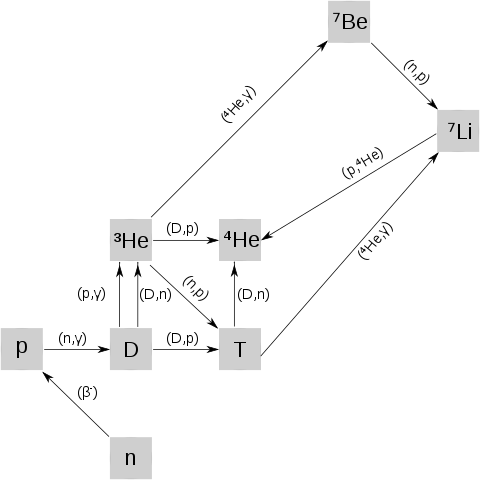
\includegraphics[width=0.8\textwidth]{figure 8.png}
    \caption{The reactions in nucleosynthesis}
    \label{fig:nsyn}
\end{figure}

The big bang theory predicted the existence of 3 kinds of neutrinos, in order for the equations to be derived and this was confirmed experimentally by the LEP experiment at CERN. The abundances of the other elements such as Hydrogen and Helium predicted from the theory also match nicely with observational evidence.

\begin{figure}[H]
    \centering
    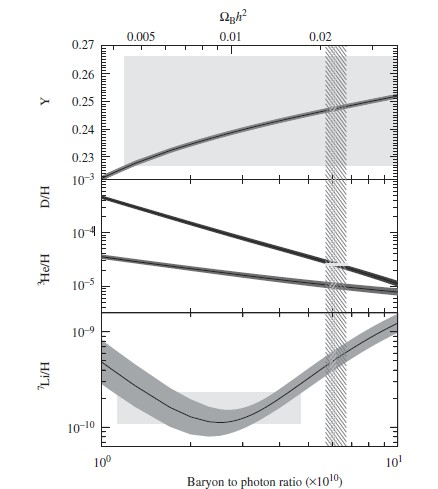
\includegraphics[width=0.8\textwidth]{figure 8.jpg}
    \caption{This plot shows the predicted abundances of light nuclei, on a scale of $\Omega_{B}h^2$ as well as baryon to photon ratio for Lithium-7, Helium-3 and Deuterium}
    \label{fig:abundance}
\end{figure}